\documentclass[border=6pt]{standalone}
\usepackage[T1]{fontenc}
\usepackage{courier}
\usepackage[scaled=0.95]{helvet}
\renewcommand{\familydefault}{\sfdefault}
\usepackage{sfmath}
\usepackage[version=4]{mhchem}
\usepackage{tikz}
\usepackage{pgfplots}
\pgfplotsset{compat=newest}
\usetikzlibrary{arrows.meta,positioning,calc,fit,backgrounds,shapes.geometric,decorations.pathreplacing,patterns}
\definecolor{ink}{HTML}{17233A}
\definecolor{inksoft}{HTML}{44506A}
\definecolor{teal}{HTML}{0E6B6B}
\definecolor{tealsoft}{HTML}{E5F0EF}
\definecolor{amber}{HTML}{B26B12}
\definecolor{ambersoft}{HTML}{FBF0DF}
\definecolor{blue}{HTML}{2F6690}
\definecolor{bluesoft}{HTML}{E3ECF4}
\definecolor{plum}{HTML}{7A4D8C}
\definecolor{plumsoft}{HTML}{EFE7F3}
\definecolor{greyc}{HTML}{8A94A3}
\definecolor{linec}{HTML}{D3DCE1}
\definecolor{oxy}{HTML}{C0392B}
\definecolor{carb}{HTML}{3B4252}
\definecolor{hyd}{HTML}{E6E9EE}
\definecolor{nit}{HTML}{2F6690}
\tikzset{
  every picture/.style={line cap=round,line join=round},
  lab/.style={font=\small, text=inksoft},
  >={Stealth[length=7pt]},
}
\pgfplotsset{
  every axis/.append style={axis line style={inksoft}, tick style={inksoft}, tick label style={font=\footnotesize, text=inksoft}, label style={font=\small, text=ink}},
}
% fragment tile: \frag{node name}{position}{colour}{content}
\newcommand{\frag}[4]{\node[draw=#3, fill=#3!12, line width=1.4pt, rounded corners=6pt, minimum width=1.25cm, minimum height=1.05cm, text=#3, font=\bfseries] (#1) at (#2) {#4};}
\newcommand{\ring}{\tikz[baseline=-0.6ex]{\draw[line width=1.1pt] (0:0.3)--(60:0.3)--(120:0.3)--(180:0.3)--(240:0.3)--(300:0.3)--cycle; \draw[line width=0.8pt] (0,0) circle (0.16);}}
\newcommand{\bond}[2]{\draw[ink, line width=2.2pt] (#1) -- (#2);}

\begin{document}
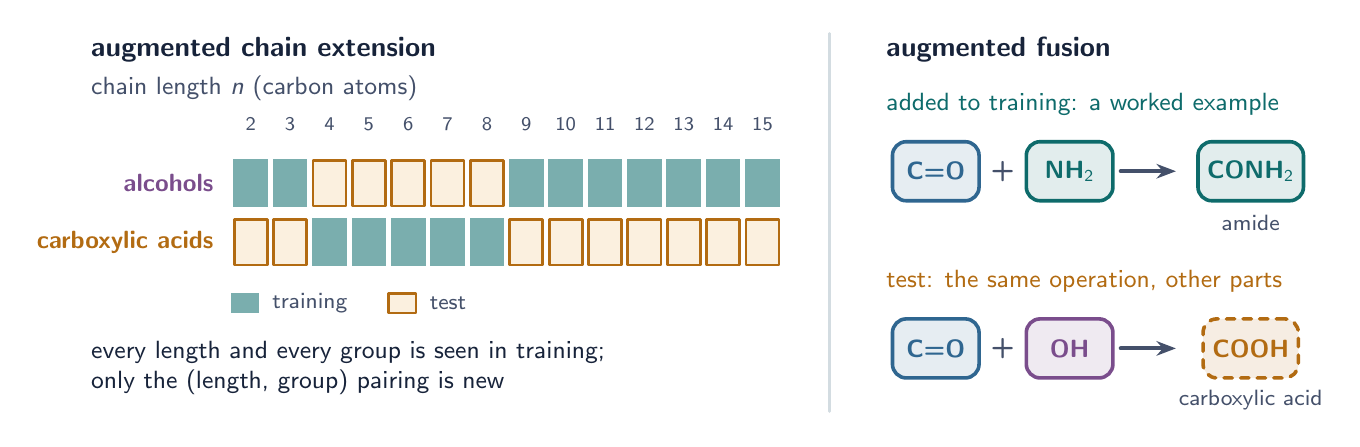
\begin{tikzpicture}
\node[font=\bfseries, text=ink, anchor=west] at (-1.9,3.3) {augmented chain extension};
\node[font=\small, text=inksoft, anchor=west] at (-1.9,2.8) {chain length $n$ (carbon atoms)};
\node[font=\scriptsize, text=inksoft] at (0.25,2.35) {2};
\fill[teal!55] (0.03,1.30) rectangle (0.47,1.90);
\draw[amber, line width=1pt, fill=ambersoft] (0.04,0.56) rectangle (0.46,1.14);
\node[font=\scriptsize, text=inksoft] at (0.75,2.35) {3};
\fill[teal!55] (0.53,1.30) rectangle (0.97,1.90);
\draw[amber, line width=1pt, fill=ambersoft] (0.54,0.56) rectangle (0.96,1.14);
\node[font=\scriptsize, text=inksoft] at (1.25,2.35) {4};
\draw[amber, line width=1pt, fill=ambersoft] (1.04,1.31) rectangle (1.46,1.89);
\fill[teal!55] (1.03,0.55) rectangle (1.47,1.15);
\node[font=\scriptsize, text=inksoft] at (1.75,2.35) {5};
\draw[amber, line width=1pt, fill=ambersoft] (1.54,1.31) rectangle (1.96,1.89);
\fill[teal!55] (1.53,0.55) rectangle (1.97,1.15);
\node[font=\scriptsize, text=inksoft] at (2.25,2.35) {6};
\draw[amber, line width=1pt, fill=ambersoft] (2.04,1.31) rectangle (2.46,1.89);
\fill[teal!55] (2.03,0.55) rectangle (2.47,1.15);
\node[font=\scriptsize, text=inksoft] at (2.75,2.35) {7};
\draw[amber, line width=1pt, fill=ambersoft] (2.54,1.31) rectangle (2.96,1.89);
\fill[teal!55] (2.53,0.55) rectangle (2.97,1.15);
\node[font=\scriptsize, text=inksoft] at (3.25,2.35) {8};
\draw[amber, line width=1pt, fill=ambersoft] (3.04,1.31) rectangle (3.46,1.89);
\fill[teal!55] (3.03,0.55) rectangle (3.47,1.15);
\node[font=\scriptsize, text=inksoft] at (3.75,2.35) {9};
\fill[teal!55] (3.53,1.30) rectangle (3.97,1.90);
\draw[amber, line width=1pt, fill=ambersoft] (3.54,0.56) rectangle (3.96,1.14);
\node[font=\scriptsize, text=inksoft] at (4.25,2.35) {10};
\fill[teal!55] (4.03,1.30) rectangle (4.47,1.90);
\draw[amber, line width=1pt, fill=ambersoft] (4.04,0.56) rectangle (4.46,1.14);
\node[font=\scriptsize, text=inksoft] at (4.75,2.35) {11};
\fill[teal!55] (4.53,1.30) rectangle (4.97,1.90);
\draw[amber, line width=1pt, fill=ambersoft] (4.54,0.56) rectangle (4.96,1.14);
\node[font=\scriptsize, text=inksoft] at (5.25,2.35) {12};
\fill[teal!55] (5.03,1.30) rectangle (5.47,1.90);
\draw[amber, line width=1pt, fill=ambersoft] (5.04,0.56) rectangle (5.46,1.14);
\node[font=\scriptsize, text=inksoft] at (5.75,2.35) {13};
\fill[teal!55] (5.53,1.30) rectangle (5.97,1.90);
\draw[amber, line width=1pt, fill=ambersoft] (5.54,0.56) rectangle (5.96,1.14);
\node[font=\scriptsize, text=inksoft] at (6.25,2.35) {14};
\fill[teal!55] (6.03,1.30) rectangle (6.47,1.90);
\draw[amber, line width=1pt, fill=ambersoft] (6.04,0.56) rectangle (6.46,1.14);
\node[font=\scriptsize, text=inksoft] at (6.75,2.35) {15};
\fill[teal!55] (6.53,1.30) rectangle (6.97,1.90);
\draw[amber, line width=1pt, fill=ambersoft] (6.54,0.56) rectangle (6.96,1.14);
\node[font=\small\bfseries, text=plum, anchor=east] at (-0.1,1.6) {alcohols};
\node[font=\small\bfseries, text=amber, anchor=east] at (-0.1,0.85) {carboxylic acids};
\fill[teal!55] (0,-0.05) rectangle (0.35,0.2); \node[font=\footnotesize, text=inksoft, anchor=west] at (0.4,0.08) {training};
\draw[amber, line width=1pt, fill=ambersoft] (2.0,-0.05) rectangle (2.35,0.2); \node[font=\footnotesize, text=inksoft, anchor=west] at (2.4,0.08) {test};
\node[font=\small, text=ink, anchor=west, align=left] at (-1.9,-0.75) {every length and every group is seen in training;\\only the (length, group) pairing is new};
\draw[linec, line width=1pt] (7.6,-1.3) -- (7.6,3.5);
\node[font=\bfseries, text=ink, anchor=west] at (8.20,3.3) {augmented fusion};
\node[font=\small, text=teal, anchor=west] at (8.20,2.6) {added to training: a worked example};
\node[draw=blue, fill=blue!12, line width=1.3pt, rounded corners=5pt, minimum height=0.75cm, minimum width=1.1cm, font=\small\bfseries, text=blue] (a1) at (8.95,1.75) {C=O};\node[font=\bfseries, text=inksoft] at (9.80,1.75) {+};\node[draw=teal, fill=teal!12, line width=1.3pt, rounded corners=5pt, minimum height=0.75cm, minimum width=1.1cm, font=\small\bfseries, text=teal] (a2) at (10.65,1.75) {NH$_2$};
\draw[->, inksoft, line width=1.5pt] (11.30,1.75) -- (12.00,1.75);
\node[draw=teal, fill=teal!12, line width=1.3pt, rounded corners=5pt, minimum height=0.75cm, minimum width=1.1cm, font=\small\bfseries, text=teal] (a3) at (12.95,1.75) {CONH$_2$};\node[font=\footnotesize, text=inksoft] at (12.95,1.1) {amide};
\node[font=\small, text=amber, anchor=west] at (8.20,0.35) {test: the same operation, other parts};
\node[draw=blue, fill=blue!12, line width=1.3pt, rounded corners=5pt, minimum height=0.75cm, minimum width=1.1cm, font=\small\bfseries, text=blue] (b1) at (8.95,-0.50) {C=O};\node[font=\bfseries, text=inksoft] at (9.80,-0.5) {+};\node[draw=plum, fill=plum!12, line width=1.3pt, rounded corners=5pt, minimum height=0.75cm, minimum width=1.1cm, font=\small\bfseries, text=plum] (b2) at (10.65,-0.50) {OH};
\draw[->, inksoft, line width=1.5pt] (11.30,-0.5) -- (12.00,-0.5);
\node[draw=amber, fill=amber!12, line width=1.3pt, rounded corners=5pt, minimum height=0.75cm, minimum width=1.1cm, font=\small\bfseries, text=amber, dashed] (b3) at (12.95,-0.50) {COOH};\node[font=\footnotesize, text=inksoft] at (12.95,-1.15) {carboxylic acid};
\end{tikzpicture}
\end{document}
